\documentclass[a4paper, 12pt]{article}

\usepackage[top=2cm, bottom=2cm, left=2.5cm, right=2.5cm]{geometry}
\usepackage[utf8]{inputenc}
\usepackage{array}
\usepackage{graphicx}

\graphicspath{{img/}}

\begin{document}
\begin{flushleft}
\includegraphics{logo}\\
\textbf{UNIVERSIDADE ESTADUAL DE PONTA GROSSA} \\
SISTEMA UNIVERSIDADE ABERTA DO BRASIL - UAB \\
\underline{Licenciatura em Matemática | Polo UAB em Jacarezinho}\end{flushleft} 
\textbf{ALUNO:} Ricardo Medeiros da Costa Junior   \textbf{RA:} 151774301 \\
\textbf{DISCIPLINA:} Fundamentos da Educação\\
\textbf{ATIVIDADE:} Atividade 7 - Tarefa: "O Pequeno príncipe e a Matemática"\\
\textbf{TUTOR(A):} Adilane de Assis Ferreira\\
\textbf{PERÍODO:} Terceiro Período \\ \\

Após a revolução científica nos séculos XVI-XVII, as transformações que abordam a noção de homem, livre de crendices e da tutela religiosa e a confiança total na razão, desenvolveu-se a preocupação com a quantificação de tudo e também do tempo. A experimentação na ciência acabou com o dogmatismo anterior fundado na metafísica, em que o argumento fundamental era o de autoridade. A partir desse momento da nossa história, o conhecimento só tem valor se ele não for abstrato e de contemplação. Desenvolve-se o projeto iluminista sustentado em três grandes bandeiras da Revolução Francesa: liberdade, igualdade, fraternidade. No entanto, a burguesia radicalizou a valorização da liberdade individual e valorizou a propriedade particular, mas colocou em segundo plano a fraternidade e a igualdade.\\
Como consequência desse período de pós-modernidade, há grande rejeição ao que é chamado de narrativas mestras ou metanarrativas, como religião, política e educação. Salienta-se que poderosas instituições como religiões milenares estão perdendo força, mais cidadãos sentem indiferença com relação a política e há ausência de disciplina e valores mínimos na escola, o que pode ocasionar em um ambiente de hostilidade e até mesmo de medo e violência.\\
Portanto, é necessário desenvolver ações pedagógicas com intuito de inserir valores na escola. Por exemplo: identificação e repúdio a situações de desrespeito promove o respeito mútuo; a valorização da justiça implica o posicionamento contrário às situações distantes no tempo e no espaço; estabelecer parcerias com instituições de saúde podem subsidiar conhecimentos para que os alunos apliquem a solidariedade caso alguém esteja passando mal e um simples desenho animado pode fazer a motivação a respeito da participação, assim, promovendo o diálogo.\\
São vários exemplo de entretenimento que podem ser usados para relacionar o pensamento matemático. Na disciplina de Instrumentação para o Ensino de Matemática I, foi mostrado um desenho da Disney, cujo é abordado a Teoria dos Números de forma significativa. Segue algumas imagens do filme \textbf{Donald no País da Matemática:}
  \begin{figure}[ht!]
    \centering
    
\includegraphics[width=80mm]{img1.png}
    \caption{Imagem 1}
  \end{figure}

  \begin{figure}[ht!]
    \centering
    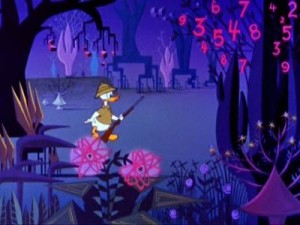
\includegraphics[width=80mm]{img2.png}
    \caption{Imagem 2}
  \end{figure}

\end{document}
